\documentclass{l4dc2026}

% The L4DC class loads amsmath, amssymb, natbib, graphicx, url, and algorithm2e.
\usepackage{bm}
\usepackage{booktabs}
\usepackage{xcolor}
\usepackage{multirow}
\usepackage{subfig}
\usepackage{times}

\newcommand{\todo}[1]{\textbf{[TODO:} #1\textbf{]}}
\newcommand{\rev}[1]{#1}
\newcommand{\calD}{\mathcal{D}}
\newcommand{\feasSet}{\mathcal{F}}
\newcommand{\AURCref}{\mathrm{AURC}_{\mathrm{ref}}}
\newcommand{\Nfive}{N_{5\%}}
\newcommand{\distdyn}{d^{\mathrm{dyn}}}
\newcommand{\placeholderfigurewide}[1]{%
    \fbox{\parbox[c][4.5cm][c]{0.96\textwidth}{\centering\small
    \textbf{FIGURE PLACEHOLDER}\\[1.5mm]#1}}}
\newcommand{\figurepdf}[2]{%
    \IfFileExists{#2}{%
        \includegraphics[width=#1]{#2}%
    }{%
        \fbox{\parbox[c][3.4cm][c]{#1}{\centering\small
        \textbf{PDF FIGURE PENDING}\\[1.5mm]\texttt{#2}}}%
    }%
}

\title[Fleet-Informed BO for Controller Calibration]{Fleet-Informed Bayesian Optimization for Data-Efficient Controller Calibration}

\coltauthor{%
\Name{Jakob Weber} \and
\Name{Markus Gurtner} \and
\Name{Adrian Trachte} \and
\Name{Andreas Kugi}\\
\addr{\textit{Draft author list -- affiliations to be finalized}}%
}

\begin{document}
\maketitle

\begin{abstract}
Controller calibration is often repeated from scratch for every new system variant, even when previously commissioned systems have already explored the same controller-weight space. We study when such historical black-box evaluations transfer across heterogeneous dynamical systems. For linear-quadratic integral (LQI) yaw-rate control, source systems provide normalized observations in a common controller-weight space that warm-start a Gaussian-process surrogate for a newly arriving system, while model identification and feedback-gain synthesis remain target-specific. Across 120 held-out target-calibration problems from 20 fleet realizations, fleet-informed Bayesian optimization reduces the budget-restricted mean number of experiments required to reach within 5\% of an independently scored system-specific reference from 6.72 to 3.08, a reduction of 54\%. All warm-started runs reach the target within the 12-experiment budget, compared with 79.2\% under independent BO. Ten historical evaluations per source recover about 93\% of the mean experiment saving obtained with 25. A dense landscape analysis explains the transfer: 99.4\% of evaluated system pairs retain Spearman rank correlation above 0.95 on jointly feasible calibration points despite substantial plant heterogeneity. Consequently, dynamics-aware source weighting provides no measurable advantage over simple pooling. The results show that a controller-calibration landscape can be substantially more invariant across systems than the underlying dynamics, making task-level calibration experience reusable for data-efficient controller commissioning.
\end{abstract}

\begin{keywords}
Bayesian optimization, controller calibration, transfer learning, data-efficient control, heterogeneous dynamical systems, LQI
\end{keywords}

\section{Introduction}
Controller calibration is an important but expensive part of commissioning modern dynamical systems. Even when the controller structure follows from model-based design, parameters such as linear-quadratic regulator or integral-control weights determine the final compromise between tracking performance, control effort, and robustness. Bayesian optimization (BO) is attractive for this setting because it can optimize low-dimensional controller parameters from a limited number of expensive closed-loop evaluations~\cite{frazier2018tutorial,marco2016lqr,berkenkamp2016safe,schillinger2017safe,vonrohr2024local}.

A fleet of related systems changes this optimization problem. Vehicles or machines are commissioned repeatedly, so previously calibrated systems have already evaluated controller parameters that a newly arriving system would otherwise have to rediscover. Reusing these observations can reduce target-system experimentation, but only if the corresponding control-performance landscapes are sufficiently aligned. Plant heterogeneity therefore creates a transfer question that is distinct from ordinary single-system BO: \emph{when are controller-calibration observations from one dynamical system informative for another?}

This question is nontrivial because the same calibration vector does not represent the same feedback gain on every plant. In the setting studied here, each system identifies its own control-design model and recomputes an LQI gain for every candidate weight vector. What is shared across systems is only the low-dimensional calibration coordinate and its observed normalized performance. Hence successful transfer requires similarity of the induced calibration objectives, not equality of the underlying dynamics or controllers.

\subsection{Related work and positioning}
BO has been used for automatic controller tuning in LQR, PI, and safety-constrained calibration problems~\cite{marco2016lqr,berkenkamp2016safe,schillinger2017safe,vonrohr2024local}. Transfer-learning BO reuses observations or surrogate information from related optimization tasks~\cite{joy2019transfer,tighineanu2022transfer,perrone2018scalable}. Federated and collaborative BO consider optimization with information distributed across agents~\cite{dai2020fts,dai2021dpfts,chen2025collaborative}, while federated control and identification exchange model or design information across heterogeneous dynamical systems~\cite{wang2026fedlqr,weber2026ifac}.

Our objective is different from proposing a new acquisition function, a common fleet controller, or a distributed GP algorithm. We use a deliberately simple pooled warm start to isolate whether historical controller-calibration observations are themselves transferable across heterogeneous plants. A dynamics-weighted variant then tests the natural hypothesis that observations from physically similar systems should be trusted more strongly. This separation lets the experiments distinguish \emph{plant heterogeneity} from \emph{calibration-landscape heterogeneity}, which is the central scientific question of the paper. Because the transferable records are compact and do not contain raw trajectories, the same formulation is compatible with distributed data ownership, but privacy mechanisms and distributed surrogate training are not contributions of this work.

The answer need not favor selective transfer. Different physical plants can induce similar rankings of the same low-dimensional LQI weight configurations even when their identified dynamics are clearly separated. If so, broad pooling should already provide effective surrogate coverage and dynamics-aware attenuation may add little. Conversely, if calibration landscapes change strongly with the plant, unweighted historical data can create negative transfer.

We evaluate these alternatives on heterogeneous nonlinear vehicle lateral dynamics. Previously calibrated source systems provide normalized controller-calibration observations. A new target begins with two local initialization experiments, combines them with the source observations, and sequentially evaluates new LQI calibrations. Only experiments executed on the target count toward its incremental commissioning cost; every candidate gain is synthesized from the target's locally identified model.

The final held-out protocol, including the compared methods, local experiment budget, primary metric, and statistical tests, was fixed before the 20 final fleet realizations were examined. The contributions are:
\begin{itemize}
    \item We formulate \emph{fleet-informed controller calibration} as transfer between related black-box control-optimization tasks. Source observations are normalized in a common three-dimensional controller-weight space, while model identification and feedback-gain synthesis remain system-specific. The evaluation explicitly separates historical source information from newly executed target experiments.
    \item In 120 held-out target-calibration problems, fleet-informed BO reduces the budget-restricted mean number of local evaluations required to reach within 5\% of an independently scored offline reference from 6.72 to 3.08. A source-maturity study shows that ten historical evaluations per source recover about 93\% of the mean experiment saving obtained with 25 evaluations per source.
    \item We characterize the mechanism behind this transfer. Despite substantial plant heterogeneity, 99.4\% of system pairs retain calibration-landscape rank correlation above 0.95 on jointly feasible points. Dynamics similarity retains a modest residual association with landscape similarity, yet dynamics-aware weighting provides no measurable improvement over unweighted pooling.
\end{itemize}

Figure~\ref{fig:concept} summarizes the cross-system calibration workflow.

\begin{figure*}[t]
    \centering
    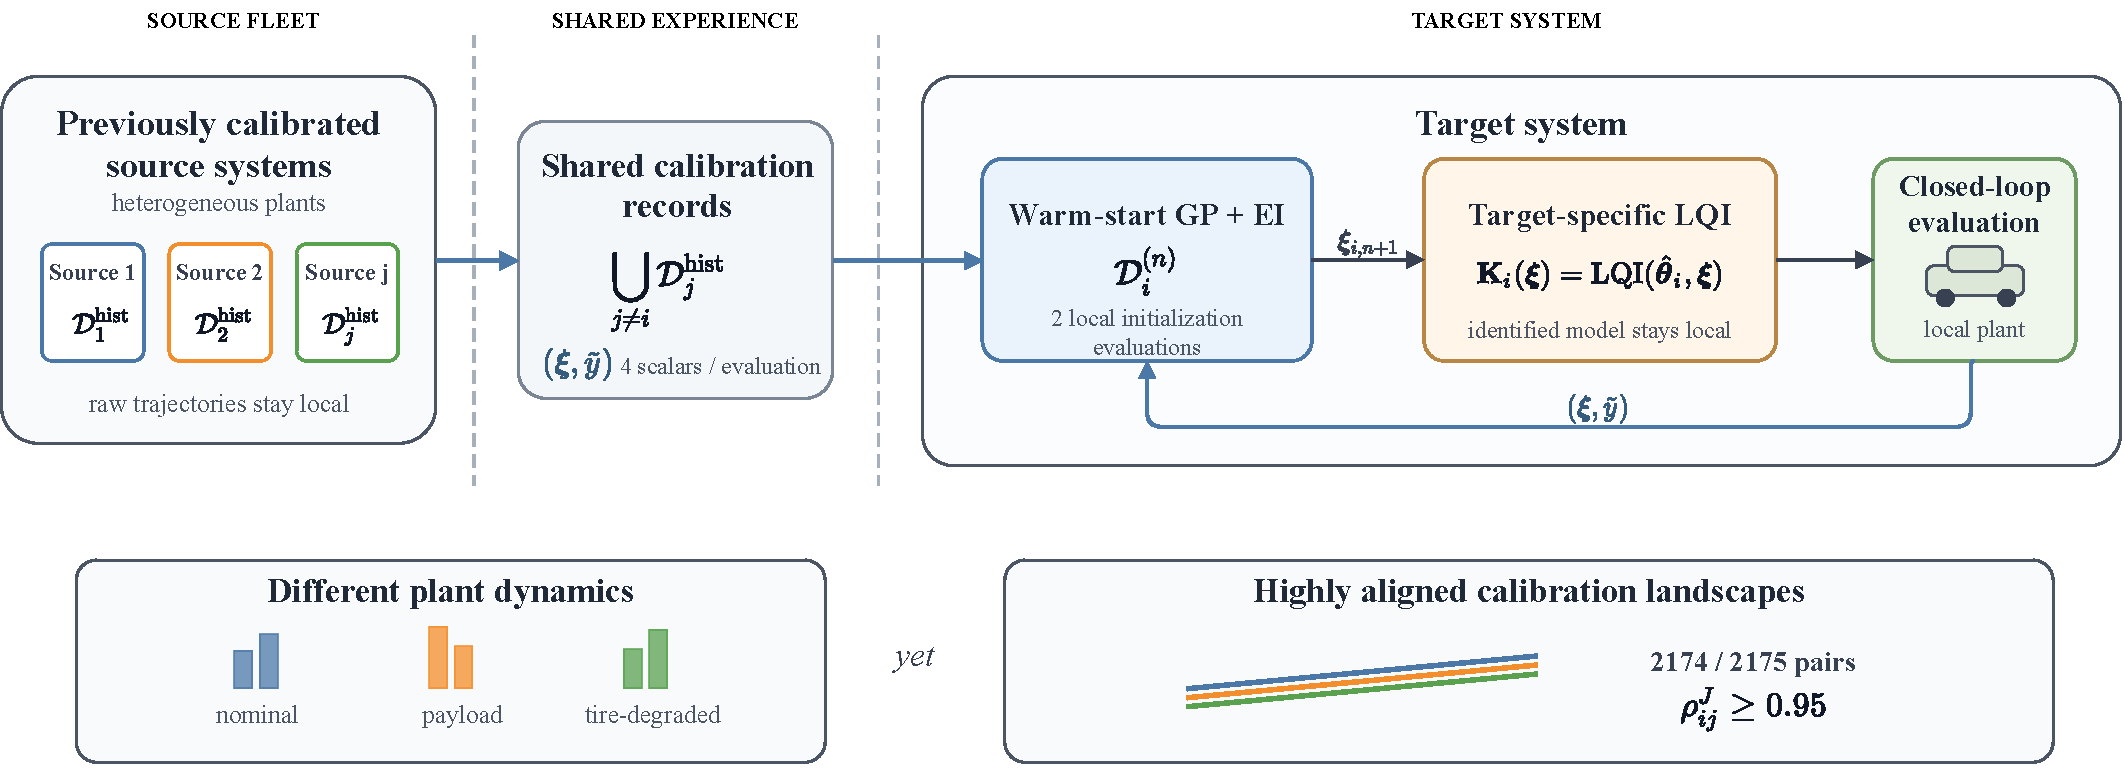
\includegraphics[width=0.96\textwidth]{figures/concept.pdf}
    \caption{Fleet-informed cross-system controller calibration. Previously calibrated source systems provide normalized observations in a common controller-weight space. These observations warm-start the BO surrogate of a newly arriving target, while model identification and LQI gain synthesis remain target-specific. Reported commissioning cost counts only closed-loop evaluations newly executed on the target; raw trajectories and source feedback gains are not required for the pooled warm start.}
    \label{fig:concept}
\end{figure*}

\section{Problem Formulation}

\subsection{Heterogeneous systems and local controller design}
Consider systems $i\in\mathcal C$ with true nonlinear plants
\begin{align}
 \mathbf{x}_{i,k+1}&=\mathbf{f}_i(\mathbf{x}_{i,k},u_{i,k},\mathbf{w}_{i,k}),\\
 \mathbf{y}_{i,k}&=\mathbf{h}_i(\mathbf{x}_{i,k},\mathbf{v}_{i,k}),
 \label{eq:true_plant_generic}
\end{align}
where $\mathbf{f}_i$ differs across systems. Each system identifies a compact linear control-design model
\begin{equation}
 \mathbf{x}_{k+1}=\mathbf{A}(\boldsymbol{\theta}_i)\mathbf{x}_k+\mathbf{B}(\boldsymbol{\theta}_i)u_k.
 \label{eq:identified_model}
\end{equation}
Local recursive least-squares identification yields the parameter estimate $\hat{\boldsymbol{\theta}}_i$ and an identification-precision matrix $\hat{\mathbf W}_i$. In the vehicle study, the state is $\mathbf{x}=[\beta,r]^\top$, where $\beta$ is vehicle sideslip and $r$ is yaw rate. The measured output used for LQI tracking is $r$, hence $\hat{\mathbf C}_i=[0\;1]$ for the identified two-state model.

For yaw-rate tracking, the state is augmented with the integral tracking error
\begin{equation}
 z_{k+1}=z_k+T_s\left(r_k^{\rm ref}-r_k\right).
 \label{eq:integral_state}
\end{equation}
With $\mathbf{x}_k^a=[\mathbf{x}_k^\top,z_k]^\top$, the LQI penalty is parameterized by the three-dimensional vector $\boldsymbol{\xi}\in\Xi\subset\mathbb R^3$. \rev{The three entries $\xi_1$, $\xi_2$, and $\xi_3$ parameterize the penalties on sideslip $\beta$, yaw rate $r$, and integral tracking error $z$, respectively.}

The augmented-state channels have different units and characteristic magnitudes. We use the fixed scale vector
\begin{equation}
 \mathbf{s}=[0.053229,\,0.575573,\,0.139862]^\top
 \label{eq:state_scales}
\end{equation}
and define
\begin{align}
 \mathbf{Q}(\boldsymbol{\xi})&=\operatorname{diag}\left(\frac{10^{\xi_1}}{s_1^2},\frac{10^{\xi_2}}{s_2^2},\frac{10^{\xi_3}}{s_3^2}\right),\\
 \mathbf{R}&=1.
 \label{eq:lqi_weights}
\end{align}
The scaling places the three state channels on comparable physical ranges, so $\boldsymbol{\xi}$ mainly controls relative penalty strength rather than compensating for different units. \rev{The numerical scales were fixed before the final BO study from representative nominal closed-loop trajectories and were not tuned separately for individual vehicle families.}

For system $i$, each candidate $\boldsymbol{\xi}$ is converted into a system-specific gain
\begin{equation}
 \mathbf{K}_i(\boldsymbol{\xi})=\operatorname{LQI}\!\left(\hat{\mathbf{A}}_i,\hat{\mathbf{B}}_i,\hat{\mathbf{C}}_i,\mathbf{Q}(\boldsymbol{\xi}),\mathbf{R}\right).
 \label{eq:lqi_gain}
\end{equation}
The same calibration vector can therefore produce a different feedback gain for every system. The transferable quantity is the location and observed performance of a calibration point in the common $\boldsymbol{\xi}$-space.

For calibration episode $\omega$, applying $\mathbf{K}_i(\boldsymbol{\xi})$ to the true plant yields the yaw-rate tracking cost $J_i(\boldsymbol{\xi},\omega)$. The system objective is
\begin{equation}
 f_i(\boldsymbol{\xi})=\mathbb E_{\omega}\!\left[J_i(\boldsymbol{\xi},\omega)\right].
 \label{eq:client_objective}
\end{equation}
Only feasible controller candidates are considered valid calibration outcomes. The feasibility conditions are defined in Sec.~\ref{subsec:vehicle_task}.

\subsection{Fleet-informed calibration objective}
A previously calibrated source system $j$ contributes the task-level calibration records
\begin{equation}
 \calD_j^{\rm hist}=\left\{\left(\boldsymbol{\xi}_{j,m},\tilde y_{j,m}\right)\right\}_{m=1}^{M_j},
 \label{eq:historical_data}
\end{equation}
where
\begin{equation}
 \tilde y_{j,m}=\frac{J_j(\boldsymbol{\xi}_{j,m})}{J_j^{\rm base}}
 \label{eq:historical_normalization}
\end{equation}
is the cost normalized by the fixed baseline controller of source system $j$. This gives historical observations from systems with different absolute tracking-error levels a common scale.

For the three-dimensional calibration vector used here, each record in $\calD_j^{\rm hist}$ contains four scalar values: the three coordinates of $\boldsymbol{\xi}_{j,m}$ and the normalized performance $\tilde y_{j,m}$. Baseline normalization makes objective values approximately commensurate across systems, while the landscape study later tests whether their ordering is preserved across heterogeneous plants. The warm start therefore transfers optimization experience rather than a source feedback gain or plant trajectory.

For a newly arriving system $i$, all historical records belonging to that same system are excluded from the source pool. This held-out construction emulates a genuinely new system and prevents leakage from a completed calibration history of the plant that is currently being calibrated.

\rev{We distinguish the incremental experimental cost $N_i^{\rm new}$, which counts only closed-loop evaluations newly executed on system $i$, from the historical pool size $N_i^{\rm hist}$, which counts source observations available before system $i$ arrives. In the final full-pool study, $N_i^{\rm hist}=29\times25=725$. The paper's sample-efficiency claim concerns a reduction in $N_i^{\rm new}$ rather than a reduction in the total number of experiments ever performed across the fleet.}

\subsection{Offline reference and threshold metric}
\rev{For reporting, each held-out system receives a high-accuracy offline reference that is computed independently of the BO decision process. The reference search first evaluates 1024 Sobol points over $\Xi=[-3,3]^3$ on the system's calibration-episode bank. The eight best feasible Sobol candidates initialize bounded Powell refinements. The best resulting calibration vector $\boldsymbol{\xi}_i^{\rm ref}$ is then scored on an independent reference-test bank containing 20 stochastic episodes per maneuver, yielding $J_i^{\rm ref}$. The reference is used only for reporting and never enters GP fitting, acquisition, normalization, or infeasibility handling. A nested convergence audit on one target from each vehicle family showed that the best 1024-point Sobol value differed from the corresponding 4096-point value by only 0.018\% on average.}

\rev{To compare the BO trajectories and the reference on the same independent evaluation distribution, every incumbent stored along each completed BO trajectory is rescored on the same reference-test bank. Let $J_{i,\mathrm{test}}^{\mathrm{best}}(n)$ denote the best independently rescored incumbent available after $n$ new-system experiments. The latent 5\% hitting time is}
\begin{equation}
 T_{i,5\%}=\min\left\{n:J_{i,\mathrm{test}}^{\mathrm{best}}(n)\le1.05J_i^{\rm ref}\right\}.
 \label{eq:n5}
\end{equation}
\rev{All runs are followed to the same local budget $B=12$. If the threshold is not reached by $B$, the hitting time is right-censored at that budget. For budget-restricted mean summaries we use $\min(T_{i,5\%},B)$, denoted by $N_{i,5\%}$ in the remainder. Under this common Type-I censoring this is the restricted mean time to threshold over the available budget. Cumulative success curves treat censored runs as unresolved rather than as successes at $B$.}

\section{Fleet-Informed Bayesian Optimization}

\subsection{Warm-started GP surrogate}
The normalization in~\eqref{eq:historical_normalization} is also applied to every observation collected by the new system. The baseline controller is fixed before BO begins and is independent of the offline reference used for reporting. Infeasible evaluations receive the same fixed penalty in normalized units.

At local evaluation $n$, the target-side optimizer or a fleet coordinator fits a GP surrogate to
\begin{equation}
 \calD_i^{(n)}=\calD_i^{\rm local}(n)\cup\bigcup_{j\ne i}\calD_j^{\rm hist}.
 \label{eq:pooled_dataset}
\end{equation}
Equation~\eqref{eq:pooled_dataset} defines a simple full-pooling transfer baseline: all available source observations are inserted directly into the target surrogate after normalization. We deliberately keep the GP model and expected-improvement acquisition rule unchanged so that any improvement can be attributed to reusing cross-system calibration information rather than to a new BO algorithm. The compact records can be communicated without source trajectories or feedback gains; distributed inference and privacy mechanisms are outside the present scope.

After initialization, the next calibration vector is selected with expected improvement~\cite{frazier2018tutorial},
\begin{equation}
 \boldsymbol{\xi}_{i,n+1}\in\arg\max_{\boldsymbol{\xi}\in\Xi}\operatorname{EI}_i\left(\boldsymbol{\xi}\mid\calD_i^{(n)}\right).
 \label{eq:ei}
\end{equation}
The new system then synthesizes $\mathbf{K}_i(\boldsymbol{\xi}_{i,n+1})$ and evaluates the controller on its own nonlinear plant. The source records remain fixed and require no additional source-system rollouts during this process.

\rev{The search region is the common box $\Xi=[-3,3]^3$. The local initialization uses two points of a Sobol low-discrepancy sequence. The source histories were generated with the same calibration coordinates and objective normalization, which allows them to be inserted directly into the new system's surrogate.}

For reproducibility, Table~\ref{tab:bo_details} summarizes the BO implementation used in the held-out study.

\begin{table}[t]
\centering
\caption{BO implementation used in the held-out study.}
\label{tab:bo_details}
\scriptsize
\begin{tabular}{@{}ll@{}}
\toprule
Quantity & Setting\\
\midrule
Search box & $[-3,3]^3$\\
Local initialization & 2 Sobol points\\
Acquisition & Expected improvement, minimization\\
EI exploration margin & $0.01$\\
EI candidate set & 256 Sobol points\\
Output scaling & $J_i/J_i^{\rm base}$\\
Source weighting floor & $0.02$\\
GP kernel & Constant $\times$ Mat\'ern-$5/2$\\
GP length scale & $\boldsymbol{\ell}_0=0.3\mathbf{1}$, bounds $[0.05,3]^3$\\
GP base noise $\alpha_0$ & $10^{-4}$\\
GP optimizer restarts & 2\\
Infeasible penalty & $3.0$ in normalized units\\
Baseline $\boldsymbol{\xi}^{\rm base}$ & $[0,\,0.30103,\,0.30103]^\top$\\
\bottomrule
\end{tabular}
\end{table}

We compare three methods. Independent BO uses only observations collected on the target system. Global fleet warm start combines all available source calibration records with equal weight and does not require source-model parameters. Dynamics-weighted warm start uses the same records but additionally uses the identified-model summaries $\hat{\boldsymbol{\theta}}_j$ and $\hat{\mathbf W}_j$ to attenuate observations from dynamically dissimilar source systems. The latter is a mechanistic ablation of the hypothesis that physical similarity predicts transfer usefulness.

\subsection{Dynamics-weighted ablation}
Because local identification provides both $\hat{\boldsymbol{\theta}}_i$ and $\hat{\mathbf W}_i$, we quantify pairwise dynamics similarity without using the latent family labels. The dynamics-weighted method therefore has access only to identified-model information and never receives the nominal, payload, or tire-degraded family identity. For systems $i$ and $j$,
\begin{equation}
(\distdyn_{ij})^2=
\left(\hat{\boldsymbol{\theta}}_i-\hat{\boldsymbol{\theta}}_j\right)^\top
\frac{\hat{\mathbf W}_i+\hat{\mathbf W}_j}{2}
\left(\hat{\boldsymbol{\theta}}_i-\hat{\boldsymbol{\theta}}_j\right),
\label{eq:dyn_distance}
\end{equation}
and
\begin{equation}
 s_{ij}=\exp\left(-\frac{(\distdyn_{ij})^2}{2\ell_d^2}\right),
 \label{eq:dyn_similarity}
\end{equation}
where $\ell_d$ is the median pairwise-distance bandwidth. Lower source similarity is converted into larger GP observation noise,
\begin{equation}
 \alpha_{ij}=\frac{\alpha_0}{\max(s_{ij},0.02)}.
 \label{eq:weighted_noise}
\end{equation}
The distance in~\eqref{eq:dyn_distance} uses the average RLS precision exactly as implemented in the confirmatory study. The GP base noise $\alpha_0$ and the remaining surrogate settings are summarized in Table~\ref{tab:bo_details}.

\section{Experimental Design}

\subsection{Vehicle model, fleet, and tracking task}
\label{subsec:vehicle_task}
The study uses a constant-speed lateral vehicle benchmark derived from the standard small-angle bicycle model~\cite{weber2026ifac}. The control-design model has state $\mathbf{x}=[\beta,r]^\top$, steering input $\delta$, and longitudinal speed $U$ that is constant within each rollout. The family prototypes use $U=15$ m/s, with small system-to-system variation described below. Its continuous-time dynamics are
\begin{equation}
 \dot{\mathbf{x}}=\mathbf{A}\mathbf{x}+\mathbf{B}\delta,
 \label{eq:bicycle_ct}
\end{equation}
with
\begin{equation}
\mathbf{A}=\begin{bmatrix}
-\dfrac{C_f+C_r}{mU} & \dfrac{-aC_f+bC_r}{mU^2}-1\\[2mm]
\dfrac{-aC_f+bC_r}{I_z} & -\dfrac{a^2C_f+b^2C_r}{I_zU}
\end{bmatrix},
\label{eq:bicycle_A}
\end{equation}
and
\begin{equation}
\mathbf{B}=\begin{bmatrix}\dfrac{C_f}{mU}\\[2mm]\dfrac{aC_f}{I_z}\end{bmatrix}.
\label{eq:bicycle_B}
\end{equation}
The model is discretized by zero-order hold with sampling time $T_s=0.05$ s.

Controller candidates are evaluated on a nonlinear version of the same lateral plant. The front and rear tire slip angles are
\begin{align}
 \alpha_f&=\delta-\beta-\frac{ar}{U},\\
 \alpha_r&=-\beta+\frac{br}{U},
 \label{eq:slip_angles}
\end{align}
and each lateral force is computed as
\begin{equation}
 F_{y,q}=\mu F_{z,q}\tanh\left(\frac{C_q\alpha_q}{\mu F_{z,q}}\right),\qquad q\in\{f,r\}.
 \label{eq:tire_nonlinearity}
\end{equation}
\rev{With static axle loads $F_{z,f}=mgb/(a+b)$ and $F_{z,r}=mga/(a+b)$, the nonlinear states evolve according to}
\begin{align}
 \dot\beta&=\frac{F_{y,f}+F_{y,r}}{mU}-r,\\
 \dot r&=\frac{aF_{y,f}-bF_{y,r}}{I_z}.
 \label{eq:nonlinear_vehicle}
\end{align}
This makes the evaluation plant intentionally more nonlinear than the model used for LQI synthesis.

The fleet contains 30 systems in every realization, with ten systems from each of three families. Table~\ref{tab:vehicle_params} lists the family prototypes. Payload systems increase mass by 20\% and yaw inertia by 25\%. Tire-degraded systems reduce front cornering stiffness by 25\%. For each generated system, $m$, $I_z$, $C_f$, $C_r$, and $U$ are independently multiplied by $1+\eta$ with $\eta\sim\mathcal U[-0.025,0.025]$, while $a$ and $b$ remain fixed at the prototype values. Thus every rollout has constant speed, but the realized speed varies by up to 2.5\% around the common 15 m/s prototype. The multiplicative range preserves positivity, so no parameter clipping is used. A generated system is resampled, using an independent deterministic random stream, if the fixed baseline controller is infeasible on the calibration task; at most 50 attempts are allowed. Family labels are used only to construct and analyze the benchmark and are not provided to BO.
\begin{table}[t]
\centering
\caption{Vehicle-family prototypes and common simulation parameters.}
\label{tab:vehicle_params}
\scriptsize
\setlength{\tabcolsep}{3.5pt}
\begin{tabular}{@{}lccc@{}}
\toprule
Parameter & Nominal & Payload & Tire-degraded\\
\midrule
$m$ [kg] & 1500 & 1800 & 1500\\
$I_z$ [$\mathrm{kg\,m^2}$] & 2700 & 3375 & 2700\\
$a$ [m] & 1.25 & 1.25 & 1.25\\
$b$ [m] & 1.35 & 1.35 & 1.35\\
$C_f$ [$\mathrm{N/rad}$] & 80000 & 80000 & 60000\\
$C_r$ [$\mathrm{N/rad}$] & 90000 & 90000 & 90000\\
$U$ [m/s] & 15 & 15 & 15\\
$T_s$ [s] & 0.05 & 0.05 & 0.05\\
$\mu$ [-] & 1.0 & 1.0 & 1.0\\
\bottomrule
\end{tabular}
\end{table}

\subsection{Identification data}
The identified control-design model is obtained locally from the same identification maneuver for every system, so the dynamics descriptor is not confounded by the balanced two-maneuver calibration task used later in BO. We estimate
\begin{equation}
 \boldsymbol{\Theta}_i=[\mathbf A_{d,i}\;\mathbf B_{d,i}]\in\mathbb R^{2\times3},
 \qquad
 \hat{\boldsymbol{\theta}}_i=\operatorname{vec}(\hat{\boldsymbol{\Theta}}_i)\in\mathbb R^6,
\end{equation}
with matrix recursive least squares using regressor $[\mathbf x_k^\top,u_k]^\top$. The estimate is initialized at the nominal discretized model, the forgetting factor is $\lambda=0.99$, and the regressor covariance starts from $\mathbf P_0=\mathbf I_3$ ($\delta=1$). Each system processes eight repeated 6 s identification episodes of the $T_{\rm lc}=1$ s lane-change reference, corresponding to 120 samples per episode at $T_s=0.05$ s. The controller used during identification is the common nominal baseline; no additional open-loop excitation is injected.

For uncertainty-aware dynamics weighting, the RLS implementation tracks an exponentially weighted innovation variance for each state row. With $\mathbf D_i=\operatorname{diag}(\hat\sigma_{i,1}^2,\hat\sigma_{i,2}^2)$ and final regressor covariance $\mathbf P_i$, the six-dimensional precision used in~\eqref{eq:dyn_distance} is
\begin{equation}
 \hat{\mathbf W}_i=\operatorname{pinv}\!\left(\mathbf D_i\otimes\mathbf P_i\right).
 \label{eq:rls_precision}
\end{equation}
This is the same precision convention used by the confirmatory implementation.

\subsection{Calibration task and feasibility}
Each BO evaluation measures yaw-rate root-mean-square error over a common pair of lane-change maneuvers. Their lane-change half-durations are $T_{\mathrm{lc}}=1.0$ s and $T_{\mathrm{lc}}=2.0$ s. Every controller candidate is evaluated on three stochastic episodes of each maneuver, giving six calibration episodes per BO query. All systems use this same balanced task distribution so that differences in the calibration objective arise from the plant rather than from different assigned maneuvers.

\begin{figure}[t]
\centering
\figurepdf{0.96\columnwidth}{figures/fig6_lane_change_reference.pdf}
\caption{Yaw-rate references used for controller calibration. Every system is evaluated on both lane-change maneuvers, and each BO query averages three stochastic episodes per maneuver.}
\label{fig:lane_change_reference}
\end{figure}

\rev{For a discrete trajectory with $T$ samples, the reported tracking metric is}
\begin{equation}
 J_i(\boldsymbol\xi,\omega)=\sqrt{\frac{1}{T}\sum_{k=1}^{T}\left(r_{i,k}(\boldsymbol\xi,\omega)-r_k^{\rm ref}\right)^2}.
 \label{eq:rmse}
\end{equation}
The two reference waveforms differ only in $T_{\rm lc}$. Before filtering, the reference is zero until $T_0=1$ s, follows a positive sine lobe of duration $T_{\rm lc}$, then a negative sine lobe of the same duration, and is zero afterward; its peak magnitude is $r_{\max}=35^\circ/$s. A zero-phase first-order Butterworth filter with 1 Hz cutoff smooths the waveform. Every episode lasts 6 s, giving $T=120$ samples at $T_s=0.05$ s. Figure~\ref{fig:lane_change_reference} shows both references.

Yaw-rate RMSE is the calibration metric. A candidate is marked infeasible if LQI synthesis fails or if the nonlinear closed-loop rollout violates the prescribed limits. The sideslip magnitude is limited to $6^\circ$. The steering-rate change is limited to $0.2618$ rad per simulation step. These feasibility conditions are applied consistently to the baseline controller, source histories, offline reference search, and new-system evaluations.

\subsection{Landscape-similarity study}
\rev{To test whether dynamics heterogeneity translates into calibration heterogeneity, all 30 systems in each of five independent fleet realizations are evaluated on the same 128-point Sobol design $\{\boldsymbol\xi^{(m)}\}_{m=1}^{128}$. For system $i$, let $\mathcal F_i$ denote the indices of feasible calibration points and let $\mathcal F_{ij}=\mathcal F_i\cap\mathcal F_j$ denote the jointly feasible subset for a pair. Pairwise landscape similarity is computed only on $\mathcal F_{ij}$,}
\begin{equation}
 \rho_{ij}^{J}=\operatorname{Spearman}\left(\{J_i(\boldsymbol\xi^{(m)})\}_{m\in\mathcal F_{ij}},\{J_j(\boldsymbol\xi^{(m)})\}_{m\in\mathcal F_{ij}}\right).
 \label{eq:landscape_similarity}
\end{equation}
\rev{This construction prevents common infeasible points from artificially increasing the rank correlation. Feasibility-set agreement is analyzed separately with the Jaccard overlap $|\mathcal F_i\cap\mathcal F_j|/|\mathcal F_i\cup\mathcal F_j|$. The study contains 2175 within-realization system pairs. Realization-level summaries are computed within each of the five fleets and then bootstrapped across fleets so that the large number of dependent pairs is not treated as independent replication.}

\begin{figure*}[t]
\centering
\subfloat[Vehicle-parameter heterogeneity.\label{fig:landscape_params}]{\figurepdf{0.475\textwidth}{figures/fig2a_vehicle_parameter_heterogeneity.pdf}}
\hfill
\subfloat[Dynamics distance versus calibration-landscape similarity.\label{fig:landscape_similarity}]{\figurepdf{0.475\textwidth}{figures/fig2b_dynamics_vs_landscape_similarity.pdf}}
\caption{\rev{Plant heterogeneity produces only limited calibration-landscape heterogeneity. Panel (a) shows the physical variation across the three vehicle families. Panel (b) shows that rank correlation remains high over the full dynamics-distance range when computed only on jointly feasible calibration points.}}
\label{fig:landscape}
\end{figure*}

\subsection{Held-out fleet-informed BO evaluation}
The final experiment uses 20 fleet realizations that were not used for method development. Each realization contains 30 previously calibrated source systems, with ten systems from each family. Every source system contributes an independent BO history of 25 evaluations. Six systems per realization, two from each family, are then treated in turn as newly arriving systems. For each such system, its own completed history is removed and the remaining $29\times25=725$ source observations are available before its calibration begins. This produces 120 held-out new-system calibration problems.

Each new system starts with $n_{\rm init}=2$ local points from a Sobol low-discrepancy sequence. The system then receives at most ten BO-selected evaluations, giving a total local budget of 12 experiments. Independent BO, global warm start, and dynamics-weighted warm start use the same local initialization and the same evaluation randomness.

The experimental accounting is intentionally asymmetric in historical information but symmetric in newly executed target experiments. Independent BO receives $N_i^{\rm hist}=0$, while both warm-start methods receive $N_i^{\rm hist}=725$ records collected before the target arrives. All three methods are allowed the same maximum $N_i^{\rm new}=12$ local experiments. This isolates the incremental value of previously accumulated optimization experience; source-history generation is not counted as free.

\rev{The primary metric is the budget-restricted $\Nfive$ defined above. As a secondary continuous metric, we use independently rescored reference-relative regret}
\begin{equation}
 r_i^{\mathrm{ref}}(n)=\frac{J_{i,\mathrm{test}}^{\mathrm{best}}(n)-J_i^{\mathrm{ref}}}{J_i^{\mathrm{ref}}}.
 \label{eq:regretref}
\end{equation}
We also report the area under this regret curve over the early local budget and fixed-budget probabilities of reaching the 5\% criterion. Fleet realization is the statistical replication unit. Metrics are first averaged over the six held-out systems in each realization, paired method differences are then formed for each of the 20 realizations, and 95\% percentile confidence intervals are obtained from 10,000 bootstrap resamples of these realization-level differences. The Wilcoxon signed-rank test is applied to the same 20 paired realization-level mean differences.

\begin{table}[t]
\centering
\caption{Final held-out evaluation protocol.}
\label{tab:protocol}
\scriptsize
\begin{tabular}{@{}ll@{}}
\toprule
Quantity & Setting\\
\midrule
Source systems per realization & 30, 10 per family\\
Held-out fleet realizations & 20\\
New systems per realization & 6, 2 per family\\
Source history per system & 25 independent BO evaluations\\
$N_i^{\rm hist}$, warm start & 725 source observations\\
Local Sobol initialization & $n_{\rm init}=2$\\
Maximum $N_i^{\rm new}$ & 12 evaluations\\
Methods & independent / global / similarity\\
Primary metric & $\Nfive$\\
\bottomrule
\end{tabular}
\end{table}

A separate nine-source coverage experiment evaluates whether the benefit depends on having all 29 source systems available. That experiment varies the number of same-family sources from five down to zero while keeping the source-pool size fixed at nine. It is used only as a robustness analysis and not for tuning the final held-out comparison. The study therefore tests whether useful cross-system transfer requires dense source coverage or persists with a substantially smaller and compositionally different source set.

\rev{We additionally perform a source-maturity sensitivity study on the same 20 held-out fleet realizations and the same six target systems per realization. For this analysis, each system's source history is generated once by independent BO from two Sobol initialization evaluations followed by sequential BO up to a total of 25 evaluations. The maturity conditions expose the exact nested prefixes $M_{\mathrm{hist}}\in\{2,5,10,25\}$, so a held-out target receives $29M_{\mathrm{hist}}\in\{58,145,290,725\}$ historical source records. Independent BO and global fleet warm start use the same target initialization, target-evaluation randomness, 12-evaluation local budget, and independently scored offline reference as the main comparison. The same fleet realizations are reused intentionally so that only source maturity changes. This experiment is therefore a sensitivity analysis rather than a second independent confirmation.}

\rev{The source-history construction differs from the main mature-fleet comparison because nested prefixes require a common two-point initialization. The main comparison uses the established mature-history protocol with eight Sobol initialization evaluations and 17 sequential BO evaluations per source system, whereas the maturity sweep uses two Sobol evaluations and 23 sequential BO evaluations. Consequently, the $M_{\mathrm{hist}}=25$ endpoint of the sensitivity study tests the same history size under a different acquisition trajectory and need not reproduce the main result exactly.}

\section{Results}

\subsection{Fleet warm start halves local experimentation}
\rev{Figure~\ref{fig:convergence} shows independently rescored reference-relative regret versus the number of new experiments performed on each held-out system. Both fleet-informed methods improve markedly faster than independent BO, while global and dynamics-weighted warm start remain nearly indistinguishable.}

\begin{figure*}[t]
\centering
\figurepdf{0.82\textwidth}{figures/fig3_confirmatory_convergence.pdf}
\caption{\rev{Held-out convergence over 20 fleet realizations and 120 new-system calibration problems after independently rescoring all incumbents on the reference-test bank. Fleet warm start accelerates controller calibration from the first BO iterations. Dynamics weighting and unweighted pooling exhibit essentially identical convergence.}}
\label{fig:convergence}
\end{figure*}

\rev{Under the strengthened reference protocol, independent BO has a budget-restricted mean time to the 5\% criterion of 6.717 local experiments, compared with 3.083 for global fleet warm start. This is a 54.1\% reduction in incremental commissioning experiments. The paired realization-level global-minus-independent difference is $-3.633$ experiments, with 95\% bootstrap CI $(-5.01,-2.37)$ and Wilcoxon $p=0.0005$. The favorable direction occurs in 15 of the 20 held-out fleet realizations and remains consistent across all three vehicle families. Independent BO reaches the criterion within the 12-evaluation budget for 95 of 120 targets, or 79.2\%, whereas both warm-start methods reach it for all 120 targets.}

\begin{table}[t]
\centering
\caption{\rev{Held-out new-system sample efficiency under the strengthened reference protocol.}}
\label{tab:main_results}
\scriptsize
\begin{tabular}{@{}lcc@{}}
\toprule
Method & Restricted mean $\Nfive$ & $P(T_{5\%}\le B)$\\
\midrule
Independent & 6.717 & 0.792\\
Global warm start & 3.083 & 1.000\\
Dynamics weighted & 3.083 & 1.000\\
\bottomrule
\end{tabular}
\end{table}

\rev{Figure~\ref{fig:n5} complements the restricted mean with the full target-attainment behavior. Panel (a) treats unresolved runs as right-censored, so the independent curve correctly plateaus below one instead of forcing censored runs to appear as successes at the final budget. Panel (b) reports success probabilities after three and five local experiments.}

\begin{figure*}[t]
\centering
\subfloat[Cumulative fraction reaching the 5\% criterion.\label{fig:n5_ecdf}]{\figurepdf{0.475\textwidth}{figures/fig4a_n5pct_ecdf.pdf}}
\hfill
\subfloat[Success probability at fixed local budgets.\label{fig:n5_success}]{\figurepdf{0.475\textwidth}{figures/fig4b_n5pct_success_probability.pdf}}
\caption{\rev{New-system experiments required to reach within 5\% of the independently scored system-specific offline reference. Panel (a) shows cumulative observed target attainment under the common 12-evaluation censoring budget. Panel (b) shows the probability of meeting the criterion within three and five local experiments.}}
\label{fig:n5}
\end{figure*}

\subsection{\rev{Moderate source-fleet maturity captures most of the benefit}}
\rev{The main comparison assumes a mature source fleet with 25 evaluations available from every peer system. Figure~\ref{fig:maturity} tests how much of the commissioning benefit remains when the available source histories are shortened. With only $M_{\mathrm{hist}}=2$ evaluations per source, the restricted mean $\Nfive$ is 6.475, close to the independent-BO value of 6.717. At $M_{\mathrm{hist}}=5$, it decreases to 5.667. The large transition occurs by $M_{\mathrm{hist}}=10$, where the restricted mean falls to 3.525 and all 120 target problems reach the 5\% criterion within the 12-evaluation budget. At $M_{\mathrm{hist}}=25$, the corresponding value is 3.283.}

\begin{figure*}[t]
\centering
\subfloat[Restricted mean $\Nfive$ versus source maturity.\label{fig:maturity_absolute}]{\figurepdf{0.475\textwidth}{figures/fig7a_fleet_maturity_absolute.pdf}}
\hfill
\subfloat[Paired mean number of local experiments saved relative to independent BO.\label{fig:maturity_savings}]{\figurepdf{0.475\textwidth}{figures/fig7b_fleet_maturity_savings.pdf}}
\caption{\rev{Sensitivity of new-system sample efficiency to source-fleet maturity. Historical source records are nested prefixes of independently generated source BO trajectories. Error bars use fleet realization as the resampling unit. Ten evaluations per source capture most of the average mature-fleet benefit, while additional source history mainly reduces the remaining tail of slower target calibrations.}}
\label{fig:maturity}
\end{figure*}

\rev{Relative to independent BO, the mean experiment saving is 0.242 evaluations at $M_{\mathrm{hist}}=2$ with 95\% CI $(-0.70,1.32)$, 1.050 evaluations at $M_{\mathrm{hist}}=5$ with CI $(-0.32,2.47)$, 3.192 evaluations at $M_{\mathrm{hist}}=10$ with CI $(1.78,4.68)$, and 3.433 evaluations at $M_{\mathrm{hist}}=25$ with CI $(2.12,4.85)$. Thus the statistically resolved benefit appears between five and ten evaluations per source. The ten-evaluation condition recovers approximately 93\% of the mean experiment saving obtained with 25 evaluations per source while using only 40\% of the per-source historical budget. The fixed-budget success probability $P(T_{5\%}\leq5)$ rises from 40.8\% under independent BO to 64.2\%, 83.3\%, and 97.5\% for $M_{\mathrm{hist}}=5,10,$ and 25, respectively.}

\rev{The sensitivity endpoint at $M_{\mathrm{hist}}=25$ yields a restricted mean of 3.283 rather than the 3.083 obtained in the main confirmatory comparison. This small difference is expected because the nested maturity experiment uses the two-plus-23 source-history construction described above, whereas the main mature-fleet comparison uses eight initialization evaluations followed by 17 sequential BO evaluations. Both protocols show a similarly large reduction relative to independent BO.}

\subsection{Dynamics-aware weighting adds no measurable benefit}
\rev{On the held-out fleets, dynamics-weighted warm start provides no detectable improvement over global pooling. The paired realization-level mean difference in budget-restricted $\Nfive$ is $0.000$ experiments with 95\% CI $(-0.05,+0.04)$ and Wilcoxon $p=1.000$. The independently rescored convergence curves in Fig.~\ref{fig:convergence} likewise remain nearly coincident.}

\rev{The mechanistic study explains why this null result is plausible without implying that dynamics information is completely irrelevant. On the 128-point jointly feasible landscape grid, 99.4\% of all 2175 system pairs satisfy $\rho_{ij}^{J}\ge0.95$, with a minimum of 0.9355. Mean rank correlation is 0.991 for same-family pairs and 0.985 for cross-family pairs, while the median feasibility-set Jaccard similarity is 1.0. Dynamics similarity $s_{ij}$ still has a modest positive association with landscape similarity. The median within-realization Spearman correlation is 0.245 with 95\% CI $(0.162,0.288)$. Thus the calibration landscapes are not exactly invariant, but the residual dependence is small relative to their uniformly high common correlation floor. This is consistent with the repeated observation that dynamics-aware weighting does not improve outcome-level sample efficiency over broad pooling. The nine-source coverage ablation in Fig.~\ref{fig:null_coverage} further shows that this conclusion does not rely on access to all 29 peers, and changing the same-family composition of the smaller source pool produces little change in global warm-start performance.}

\begin{figure*}[t]
\centering
\subfloat[Held-out global versus dynamics-weighted warm start.\label{fig:null_pairwise}]{\figurepdf{0.475\textwidth}{figures/fig5a_global_vs_weighted_parity.pdf}}
\hfill
\subfloat[Sensitivity to same-family source coverage.\label{fig:null_coverage}]{\figurepdf{0.475\textwidth}{figures/fig5b_coverage_sensitivity.pdf}}
\caption{Dynamics-aware source weighting does not improve new-system sample efficiency. Panel (a) compares global and weighted warm start on the held-out fleets. Panel (b) shows that their performance remains similar when same-family source coverage is deliberately reduced.}
\label{fig:null_weighting}
\end{figure*}

\subsection{Continuous early-budget performance}
\rev{The 5\% threshold is intentionally easy to interpret, but it still selects one performance level. We therefore use the area under the independently rescored reference-relative regret curve as a secondary continuous measure of early calibration progress. Figure~\ref{fig:convergence} shows the same ordering as the threshold metric: both warm-start methods reduce regret substantially earlier than independent BO, while global and dynamics-weighted transfer remain nearly indistinguishable. The agreement between the threshold-based and continuous views shows that the sample-efficiency conclusion is not an artifact of the 5\% criterion.}

\section{Discussion}
\rev{The main practical conclusion is that an existing fleet should be treated as a reusable source of controller-calibration information. In the studied LQI problem, a newly arriving system reaches near-reference performance after roughly three local experiments when historical fleet observations are available, compared with a budget-restricted mean of 6.7 experiments under independent BO. All 120 warm-started target problems reach the 5\% criterion within the 12-evaluation budget, whereas 20.8\% of the independent runs remain unresolved at that point.}

\rev{The source-maturity sweep qualifies this conclusion in an important way. A minimally populated history is not sufficient by itself. At $M_{\mathrm{hist}}=2$, the paired confidence interval still includes no benefit over independent BO, and the five-evaluation condition remains statistically unresolved. By ten evaluations per source, however, the restricted mean has already fallen to 3.525 and all targets reach the criterion within budget. The additional reduction from ten to 25 source evaluations is small in the restricted mean, although the deeper history still improves reliability, with $P(T_{5\%}\leq5)$ increasing from 83.3\% to 97.5\%. The practical interpretation is therefore not that any amount of fleet history suffices. Rather, moderate source maturity captures most of the average commissioning-speed benefit, while deeper histories reduce the remaining tail risk and improve final reference-relative regret.}

\rev{The weak $M_{\mathrm{hist}}=2$ result is also mechanistically plausible. Those source histories contain only the common two-point Sobol initialization, so the nominal total of 58 source observations represents repeated evaluations at only two calibration locations across the fleet. Sequential BO then diversifies the source trajectories and increases calibration-space coverage. The strong transition between five and ten evaluations per source is consistent with this shift from repeated initialization information toward broader source-space coverage.}

\rev{The more surprising result concerns heterogeneity. The vehicle families differ in mass, yaw inertia, and tire properties, and Fig.~\ref{fig:landscape} shows that their identified dynamics are clearly distinguishable. Nevertheless, these differences translate into only limited changes in the ordering of LQI calibration settings. On the denser jointly feasible landscape study, 99.4\% of system pairs remain above $\rho_{ij}^{J}=0.95$. A modest residual relationship with dynamics similarity remains, so plant and calibration heterogeneity are not completely decoupled. For the fixed-speed, three-parameter LQI calibration problem and maneuver family studied here, however, that residual dependence is too small to yield a measurable advantage for dynamics-weighted transfer. This interpretation should not be generalized to higher-dimensional controller classes, different operating conditions, or arbitrary heterogeneous plants without further evidence.}

\rev{This observation also explains why simple pooling performs so well. In a three-dimensional search space with little new-system data, additional historical observations improve GP coverage even when they originate from dynamically different systems. The result should not be read as evidence that dynamics similarity contains no information. Rather, the remaining calibration-landscape differences are small relative to the strong cross-system agreement, so selectively attenuating dynamically dissimilar records does not improve commissioning efficiency in the investigated benchmark.}

The experiments also identify a useful level of abstraction for transfer. In this problem the reusable object is neither the plant model nor the feedback gain, but the task-level calibration record $(\boldsymbol{\xi},\tilde y)$. At the practically relevant maturity level $M_{\mathrm{hist}}=10$, each target receives 290 such records from 29 sources, with four scalars per record. The important result is not communication optimality, but information sufficiency: these compact observations preserve enough cross-system objective structure to reduce target experimentation substantially. Their compactness also permits implementations in which raw trajectories remain local, although communication protocols and privacy guarantees are not studied here.

The historical source records are not free. Each was generated by experiments performed when earlier systems were commissioned. The economic argument is instead one of reuse. Once these evaluations have been collected, their cost can be distributed across subsequent systems. \rev{Accordingly, the reported 54\% reduction is a reduction in incremental new-system commissioning experiments, not a 54\% reduction in total fleet-wide data generation.}

Several limitations remain. Validation is simulation based. The nonlinear evaluation plant is intentionally mismatched to the controller-design model, but real-vehicle confirmation is still missing. The study considers one controller structure, one three-dimensional calibration parameterization, one narrow constant-speed operating regime, and one lateral tracking application. There is no theorem guaranteeing that calibration-landscape alignment persists for higher-dimensional controller classes or more heterogeneous tasks; such settings may also make selective or multi-task BO models more valuable than simple pooling. The dense offline reference is numerically well converged and independently scored, but it remains a numerical reference rather than a proof of the global optimum. Finally, our goal is to characterize transferability and sample efficiency, not to propose a privacy-preserving or communication-optimal distributed BO protocol.

\section{Conclusion}
This paper studied when controller-calibration experience transfers across heterogeneous dynamical systems. A simple fleet-informed BO warm start reuses normalized historical observations in a common LQI weight space while retaining system-specific model identification and gain synthesis. Across 120 held-out vehicle calibration problems, this reduces the budget-restricted mean number of target experiments required to reach within 5\% of an independently scored reference from 6.72 to 3.08, and ten historical evaluations per source recover about 93\% of the mean saving obtained with 25. The mechanistic result is equally important: although the vehicle dynamics are heterogeneous, 99.4\% of system pairs retain calibration-landscape rank correlation above 0.95 on jointly feasible points. This explains why dynamics-aware source weighting does not improve over simple pooling in the studied regime. The experiments therefore support a distinction between plant heterogeneity and task-landscape heterogeneity: for data-efficient controller commissioning, the latter determines whether cross-system optimization experience is reusable.

\bibliography{references}

\end{document}
